\section{Iterative learning control}
Iterative learning control is an effective scheme used to improve repeatedly executing system performance \cite{ILC:2018}. Since torque pulsations were found to be periodic, ILC can be used to learn from previous iterations, thus making it possible to identify torque pulsations automatically. ILC based compensator can be used to reduce the ripple with weak process knowledge \cite{ILC:2007}, which makes the method well suited when numerous systems require compensation.


\subsection{ILC prerequisites}
For ILC to be effective, the following postulates must hold \cite{ILC:Book2007, ILC:2012, ILC:1998}
\begin{itemize}
  \item[1)] Every iteration ends in a fixed time duration.
  \item[2)] System invariance is ensured throughout repetition.
  \item[3)] The system output is measured in a deterministic way.
\end{itemize}
In addition to previous postulates, a few system related considerations should be accounted. The measured speed (or torque) must not be filtered too heavily, as this introduces compensation delay. Too great delay can annihilate applied compensation. Since ILC learns from previous iterations, memory storage is required. The memory is accessed frequently, which advocates use of random access memory (RAM). The required memory size depends on compensation accuracy that is being pursued. In addition to free memory space, also processing power is needed for computing compensation values.


\subsection{Ripple minimization concept}
The torque pulsations can be negated by generating an opposing torque. This can be done by computing a correction term, which is injected to a control reference. Ideally, the term has the same magnitude but opposite sign as pulsating torque at some time instant. This creates destructive interference which cancels out pulsations.

Disturbances were found to be periodic, which allows them to be identified iteratively. Identification can be done comparing the measured output value with the reference value. In practice, an error can be calculated by subtracting the measured speed from the speed reference and then the task of ILC is to minimize the error by injecting an appropriate correction term. The correction value can be injected either into torque reference \cite{ILC:2004} or to q-axis current reference \cite{ILC:2005, ILC:2018} similarly to Fig. \ref{Compensator_control_diag}. ILC tracks complete periods, which allows it to iteratively find appropriate correction terms for every step.

The minimization concept is easy to understand from examples. A simulation result in Fig. \ref{fig:ilc_concept} shows compensation of arbitrary pulsations. The green signal in plots represents torque produced by the ILC compensator. The blue signal is the pulsating torque, which represents only the sixth harmonic for the sake of clarity. Pulsations are summed to ideal electromagnetic torque, thus leading oscillations of the red signal. Since ILC is disabled in the upper plot, no compensating torque is produced and torque pulsations are directly visible from the actual torque. In the lower plot, ILC is enabled and compensating torque is produced. Now actual torque has smaller amplitude than pulsating torque, which allows to deduce that the compensator reduces torque pulsations. It can be observed that the compensating signal has roughly the same amplitude as actual torque in the upper plot while the phases differ by $\pi$. As a result, majority of torque pulsations cancel out. Part of pulsations remain due to introduction of robustness coefficient \cite{ILC:1990, ILC:2004, ILC:2005}, which will be explained later.
\begin{figure}[htb] 
    \centering
    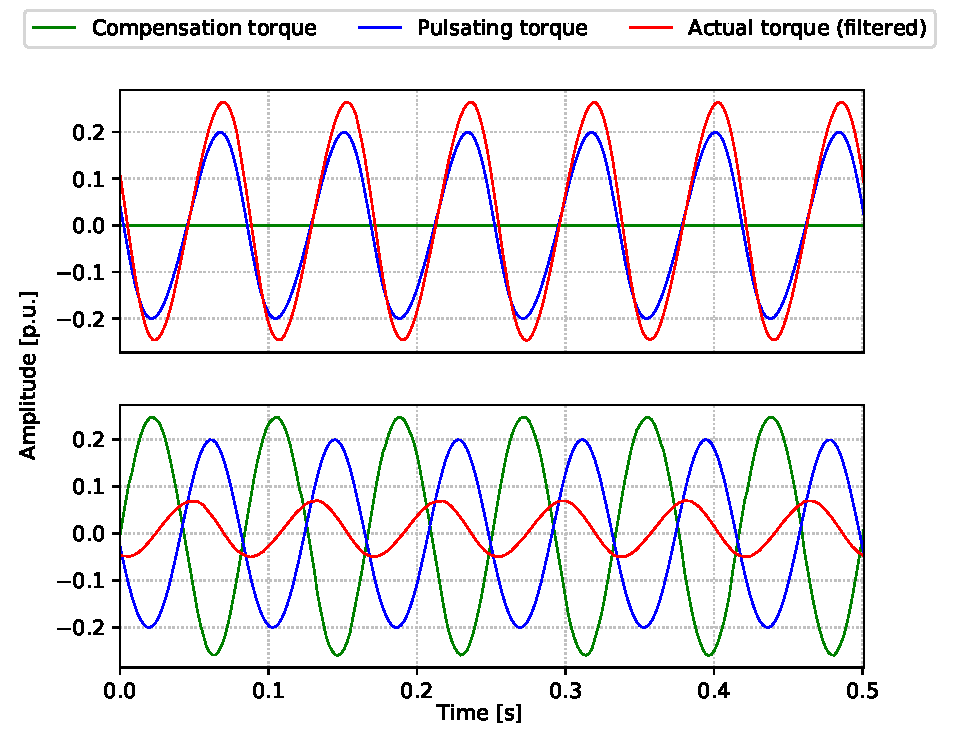
\includegraphics[width=\textwidth]{images/ilc-concept.pdf}
    \caption{The upper figure shows arbitrary torque pulsations, that are reduced in the lower figure, due to simulated destructive interference caused by the ILC compensator}
    \label{fig:ilc_concept}
\end{figure}

Figure \ref{fig:ilc_concept2} illustrates retrieval and improvement process of compensation values. Previous iteration execution is shown with dashed lines, whereas solid lines correspond to current iteration. Compensation torque has been too small on the previous iteration, thus letting the speed to oscillate and induce error between the reference and the measured value. ILC has detected the speed error and it is improving the compensation waveform by increasing amplitude of the compensation pattern. The old compensation values are getting replaced with new values. Due to improved compensation, the speed oscillations have gotten smaller on the current iteration. The ILC compensator is able to retrieve compensation values consistently from the memory by utilizing measured rotor angle. The compensation pattern consists of numerous discrete values that are saved into the memory. It will be discussed how the compensation values can be computed mathematically in the next subsection.
\begin{figure}[htb] 
    \centering
    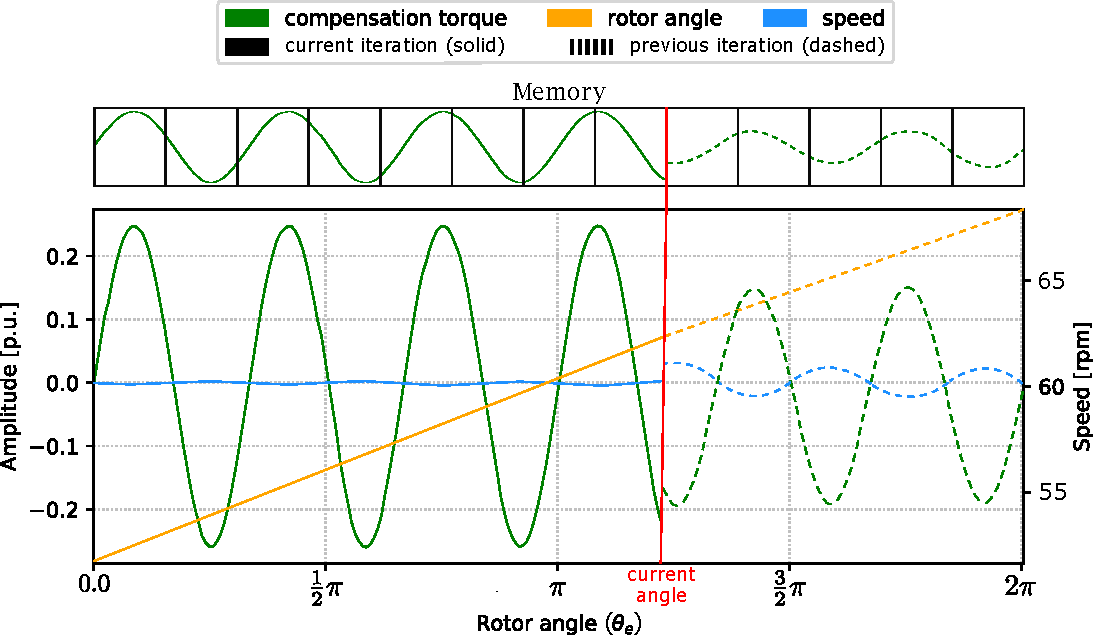
\includegraphics[width=\textwidth]{images/compensation-scheme.pdf}
    \caption{Iterative learning concept of the ILC compensator}
    \label{fig:ilc_concept2}
\end{figure}


\subsection{Iterative learning control algorithm}
ILC is not a single algorithm, but instead, a methodology consisting of many update laws. The vast majority of ILC literature focuses on either proportional type (P-type) or derivative type (D-type) update laws \cite{ILC:1998}. Since unnecessary noise build-up in this problem can be avoided by selecting the P-type update law over the D-type \cite{ILC:2005, ILC:2018}, the focus shall be on a P-type learning controller. In addition, various P-type controllers have been already applied successfully for the speed ripple minimization problem \cite{ILC:2004, ILC:2005, ILC:2012, ILC:2018}.

The learning law is given by \cite{ILC:2005, ILC:2004}
\begin{equation}
    u_{i}(\theta) = (1 - \alpha)u_{i-1}(\theta) + \Phi e_{i-1}(\theta) + \Gamma e_{i}(\theta)
    \label{ILC_update_law2}
\end{equation}
where $\theta$ is the rotor angle, which can be either mechanical or electrical as there is relation between the two. $\Phi$ and $\Gamma$ are gains used to tune controller, $e$ is the speed error and $u$ is control action, which in this case corresponds the current reference correction signal $i^{corr}_{q,i}$. The iteration index $i = 1,2,3,...$ corresponds either mechanical or electrical period depending on whether mechanical or electrical rotor angle is used. The first measurable error is $e_i$ and $e_{i-1}$ can be obtained from memory after one period. Values in the memory can be initialized to zero \cite{ILC:2004}. Figure \ref{fig:ILC_angle_block} visualizes the structure of the ILC algorithm.
\begin{figure}[b]
    \centering
    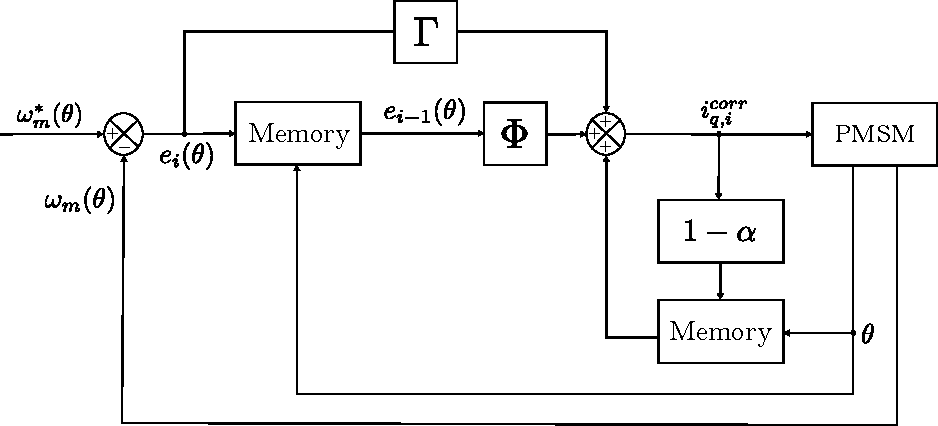
\includegraphics[width=1.0\linewidth]{images/Angle_based_ILC.pdf} 
    \caption{Block diagram of rotor angle-based ILC}
    \label{fig:ILC_angle_block}
\end{figure}

Forgetting factor $\alpha$ can be used to make the P-type algorithm more robust against noise, initialization error and system dynamics fluctuation \cite{ILC:1990, ILC:2005}. Therefore, the parameter $\alpha$ is included into learning law, as this is expected to improve the performance of the controller with real systems. For the same reason, also present error signal $e_{i}(\theta)$ is included, in addition to typical previous iteration error $e_{i-1}(\theta)$, as this should stabilize the learning in presence of perturbations \cite{ILC:2004}.

The memory usage can be adjusted as long as the memories hold values at least for one full period. Since period length depends on running speed, this leads to the situation where different memory sizes would be needed for different speeds, if memories were accessed with time directly. For this reason, the update law is written with respect to rotor angle, as this allows to have fixed memory size. By quantizing one period into $N$ steps, the values can be stored into memory holding $N$ values. Thus, step size selection has direct effect to memory consumption as well as to compensation performance. The performance suffers if steps are too large, since the algorithm cannot track error accurately.

The fixed size memory is accessed by utilizing rotor angle. Rotor angle quantized to $k$ indices is given by, i.e., $\theta_k = 2\pi k / N$ \cite{ILC:2012}. The measured rotor angle can be associated to an index by using rounding rule, $k = $round$(N \theta / 2 \pi)$ \cite{ILC:2012}. Use of the index $k$ allows reading and writing to desired memory locations. The same element can be consistently retrieved from the memory every period, hence allowing improvement to happen iteratively. It should be noted that quantization makes it possible to leap over values, especially in case of high speed and many steps. The skipped values should be linearly interpolated \cite{ILC:2012}.

The gain values $\Phi$ and $\Gamma$ should be selected carefully to allow converge. Convergence condition for the controller can be derived starting from the torque equation \eqref{torque_eq3} and the final condition is given as \cite{ILC:2004}
\begin{equation}
    \left| \rho \right| = \left| \frac{1-\alpha - k_t \Phi}{1 + k_t \Gamma} \right| < 1
\end{equation}
Since $k_t$ > 0, the condition is satisfied with \cite{ILC:2004}
\begin{equation}
    0 < \alpha + k_t \Phi < 2
\end{equation}
If the torque constant $k_t$ is unknown, its upper bound must be estimated in order to set a value for $\Phi$. Prudent upper bound estimate guarantees convergence for a wider range of $k_t$, but also leads to slower convergence rate \cite{ILC:2004, ILC:2005}. Finding a good value for $\Phi$ is important as it considerably affects the compensation performance. The gain $\Gamma$ influences compensator response between iterations \cite{ILC:2005}. Too large $\Gamma$ will cause oscillatory response, hence, a prudent estimate of $\Gamma \leq \Phi$ may suffice for producing satisfying results \cite{ILC:2004}. However, better compensation performance can be achieved by carefully tuning the controller, instead of using the prudent tuning guidelines.

It can be speculated whether the use of mechanical rotor angle in ILC could provide better compensation results than electrical rotor angle. Mechanical rotor angle allows ILC to observe all possible manufacturing imperfections occurring on one full rotation. Electrical period is only a fraction of mechanical, so asymmetry between poles cannot be fully accounted. However, a shorter period allows to have smaller memory sizes and theoretically ILC should learn faster, because iterations take less time. This gives a good reason to favor electrical angle over the mechanical. During experimental tests, it was observed that use of electrical angle also allows to set slightly higher ILC gains, before instability is encountered. As a direct consequence, the implementation using electrical rotor angle performed slightly better than identical mechanical rotor angle based implementation.

% ILC citations:
% Arimoto        ILC:1984
% Book           ILC:1998
% P-type         ILC:1990
% Panda 1st      ILC:2004
% Panda 2nd      ILC:2005
% ILC survey     ILC:2007
% Angle-based    ILC:2012
% Airplane grid  ILC:2013
% Robust ILC     ILC:2018

\clearpage
